\section{Exploration vs. Exploitation}
\begin{frame}{Exploration vs. Exploitation}

\begin{figure}[ht]
  \centering
  \begin{tabular}{c c}
      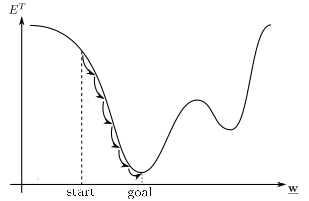
\includegraphics[height=3.5cm]{img/gradient-descent.pdf} &
      \includegraphics[height=3.5cm]{img/gradient-descent_local.pdf}
  \end{tabular}
  \caption{Learning by gradient descent}\label{fig:graddescent}
\end{figure}

\notesonly{
%An
%introduction illustrating the underlying analogy can be found in
%\textcite[ch. 7]{DudaEtAl2001}.  \textcite{Murphy2012} gives a good
%and extensive discussion of undirected graphical models (Markov Random
%fields, ch~19), variational inference (ch~21; mean field for the ISING
%model, ch~21.3), and Monte Carlo Methods (ch~23), as well as MCMC
%methods (ch~24). Further information regarding variational methods can
%be found in \textcite{Bishop2006}.

Learning is about tuning model parameters to fit some objective given training data. 
For simple models with only few parameters one can formulate an analytic solution that optimizes the objective and yields the optimal parameters directly. 
A soon as the number of parameters increases we opt for iterative gradient-based methods for finding the extrema of the objective function. If we were trying to minimize some cost function $E$, 
iteratively updating the parameters $\vec w$ by moving them in the direction of where the gradient points steepest leads to the location of an extremum. 
However, the cost function may contain multiple extrema, and there is no guarantee gradient-based learning will take us to a \emph{global} or \emph{local} optimium. 
Following the gradient assuming that it will lead to a solution that represents the global optimum is considered a \emph{greedy} approach to learning. 

Completly abandoning such assumptions will lead to a \emph{random search} for the optimal parameters. When the previous set of paramters has no influence on the choice of weights in the next iteration, 
then our learning approach is dominated by \emph{exploration} as opposed to \emph{exploitation} when we learn in a greedy fashion.
}

\end{frame}

\begin{frame}{Exploration vs. Exploitation}

\begin{figure}[ht]
  %\centering
  \begin{tabular}{c c}
		exploration & exploitation\\
      \includegraphics[height=3.0cm]{img/exploration.pdf} &
      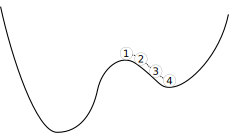
\includegraphics[height=3.0cm]{img/exploitation.pdf}\\
      random search & greedy search/hill ``climbing''
      \end{tabular}
  \caption{exploration vs. exploitation}
  \label{fig:exploration-exploitation}
\end{figure}

\pause

\question{What are the advantages and disadvantages of exploration?}

\notesonly{
The advantage of exploration is that we always discard a set of paramters if the next set yields a better cost value. Therefore, exploration is not prone to getting stuck inside a local optimum. The obvious disadvantage is that there are no guarnatees on how long it will take to find the global optimum. We never know if we've converged or not. Exploitation, or the greedy approach (with the approprate learning rate schedule) is able to converge. However, wether it reaches a global or local solution depends on the starting position.
}


\end{frame}

%\underline{Motivation 1:} We will look at how stochastic optimization can find a tradeoff between the two modes exploration and exploitation.
